\documentclass[11pt,letterpaper,oneside]{book}
\usepackage[utf8x]{inputenc}
\usepackage{amsmath}
\usepackage[spanish, es-tabla]{babel}
\usepackage{amsfonts}
\usepackage{amssymb}
\usepackage{multirow, array} 
\usepackage{chngcntr}
\usepackage{graphicx}
\usepackage{subfig}
\usepackage{cite}
%\usepackage{apacite}
\title{}
\begin{document}
\begin{center}
\thispagestyle{empty}
\fontsize{11pt}{11pt}\selectfont 

%%%%%%%%%%%%%%%%%%% PORTADA %%%%%%%%%%%%%%%%%%%%%%%%
PLAN DE TRABAJO DE GRADO 

\vspace{3cm}


\textbf {DISEÑO E IMPLEMENTACIÓN DE UN SISTEMA DE  CARACTERIZACIÓN PARA LOS FOTOMULTIPLICADORES DE SILICIO (SIPM) DEL TELESCOPIO DE MUONES (MUTE)}


\vspace{3cm}

{ Autor}
\\
{JUAN CARLOS SÁNCHEZ VILLAFRADES}

\vspace{2cm}
{ Director}
\\
{ JESÚS PEÑA RODRÍGUEZ\\M.Sc. en Ing. Electrónica}\\
\vspace{2cm}
{ Codirector}\\
{ LUIS ALBERTO NÚÑEZ DE VILLAVICENCIO MARTÍNEZ}\\ Ph.D. en Física \\
\vspace{2cm}
{ ESCUELA DE INGENIERÍAS ELÉCTRICA, ELECTRÓNICA Y TELECOMUNICACIONES
}\\
{ UNIVERSIDAD INDUSTRIAL DE SANTANDER}\\
{ BUCARAMANGA}\\
{ 2018}

  \end{center}
\large

%%%%%%%%%%%%%%%%%%%%%%%%%%%%%%%		TABLA DE FIRMAS
\newpage
\begin{center}
\thispagestyle{empty}
\begin{table}[h!]
\centering
\begin{tabular}{|l|l|l|}
\hline
 ELABORADO POR:                                                         & REVISADO POR:                                                           & APROBADO POR:                                                                                                                                                                     \\ \hline \hline
\begin{tabular}[c]{@{}l@{}} \\ \\ \\ \\ \rule{40mm}{0.2pt} \\ \scriptsize{Juan Carlos Sánchez Villafrades}\\ \tiny{\textit{Estudiante de Ingeniería Electrónica}}\\ \tiny{\textit{Código UIS:  2120566 }} 
\end{tabular} 
& \begin{tabular}{@{}l@{}} \\ \\ \\ \\ \rule{40mm}{0.2pt} \\ \scriptsize{M.Sc. Jesús Peña Rodríguez } \\ \tiny{\textit{Director del trabajo de grado}}\\ \\ \end{tabular}       
& \begin{tabular}{@{}l@{}} \scriptsize{Comité de trabajos de grado E\textsuperscript{3}T}\\ \scriptsize{Acta no. \rule{10mm}{0.2pt} del \rule{10mm}{0.2pt} de}\\ \scriptsize{\rule{20mm}{0.2pt} de 2018}\\ \scriptsize{código del trabajo:\rule{20mm}{0.2pt}}\\ \\ \\ \rule{40mm}{0.2pt}\\ \scriptsize{Evaluador designado por el comité}
\end{tabular} \\ \hline
&\begin{tabular}{@{}l@{}} \\ \\ \\ \rule{40mm}{0.2pt} \\ \scriptsize{Ph.D. Luis Alberto Núñez }\\\scriptsize{ de Villavicencio Martínez}  \\ \tiny{\textit{Codirector del trabajo de grado}}\\ \\ 
\end{tabular} &                                                                                                                                                                                   \\ \hline
\end{tabular}
\end{table}
\end{center}


\noindent\makebox[\textwidth][c]{%
\begin{minipage}[b][8cm][c]{10cm}
\begin{center}
\textbf{Universidad Industrial de Santander (UIS)\\Documento Confidencial\\}
\end{center}
%\begin{center}
\scriptsize{Ni la totalidad ni parte de este documento puede reproducirse, almacenarse o transmitirse por algún procedimiento electrónico o mecánico, incluyendo fotocopias, grabación magnética o electrónica o cualquier medio de almacenamiento de información y sistemas de recuperación, sin permiso escrito de la UNIVERSIDAD INDUSTRIAL DE SANTANDER.\\Este es un documento interno de la UIS.  Al recibirlo no podrá pasarlo a persona alguna excepto las que se le indique en la lista de distribución autorizada por la UIS. Cualquier persona externa a la UIS que utilice la información en este documento asume la responsabilidad por su empleo.\\}
%\end{center}
\begin{center}
\textbf{© Universidad Industrial de Santander (UIS) – 2018}
\end{center}

\end{minipage}}
%%%%%%%%%%%%%%%%%%%%%%%%%%%%%%%% GLOSARIO %%%%%%%%%%%%%%%%%%
\newpage
\chapter*{Glosario}
\begin{description}
	\item[APD:] Fotodiodo de avalancha (Por sus siglas en inglés Avalanche photodiode). Es un fotodiodo de alta sensibilidad y velocidad que internamente multiplica una fotocorriente cuando un voltaje inverso es aplicado \cite{Apd_Hamamatsu}. 
    
    \item[CORRIENTE OSCURA:] Es una de las principales fuentes de ruido de un SIPM, su principal componente son los portadores generados térmicamente en las uniones PN, también llamados pulsos oscuros \cite{Intro_SIPM_Sensl}. Estos pulsos no son distinguibles de los pulsos generados por fotones \cite{Apd_Hamamatsu}.      
	
    \item[GIRG:] Grupo de Investigación en Relatividad y Gravitación de  la escuela de Física de la Universidad Industrial de Santander (UIS).   
	
    \item[HODOSCOPIO:] Es un instrumento utilizado para detectar el paso de partículas cargadas y determinar su trayectoria. Los hodoscopios se caracterizan por estar formados por muchos segmentos que permiten inferir por donde pasó la partícula a través del hodoscopio \cite{Hodoscope}.     
	
    \item[MUÓN:] Es una partícula elemental, negativamente cargada, similar al electrón pero con mucho más masa \cite{Muon_wiki}. Tiene una vida media de aproximadamente 2.2 $\mu$s \cite{muon}.
    
	\item[MUTE:] Telescopio de Muones para Muongrafía Volcánica. Es un telescopio de muones que se busca construir, apto para aplicación de técnicas de tomografía de muones en diferentes escenarios geofísicos, con principal interés en el estudio de estructuras internas de volcanes de alta peligrosidad como el Volcán Cerro Machín (Tolima). El telescopio MuTe combina de manera innovadora la detección de partículas por centelleo y por producción de radiación Cherenkov en agua, obteniendo un detector híbrido de muones.           

	\item[PHOTOELECTRON (p.e.):] Es Un pulso de corriente como respuesta de una descarga de una única microcelda del SIPM.    
       
	\item[SIPM:] Fotomultiplicadores de silicio (Por sus siglas en inglés Silicon Photomultiplier). Es un dispositivo opto-semiconductor conformado por múltiples APD operando en modo Geiger. Permite la detección de señales luminosas de baja potencia. Con la ventaja de operar con bajo voltaje ($\sim 50V$) y ser inmune a los campos magnéticos \cite{Intro_SIPM_Sensl}.   

\end{description}

%%%%%%%%%% CONTENIDO %%%%%%%
\newpage
\tableofcontents % indice de contenidos

\cleardoublepage
\addcontentsline{toc}{chapter}{Lista de figuras} % para que aparezca en el indice de contenidos
\listoffigures % indice de figuras

\cleardoublepage
\addcontentsline{toc}{chapter}{Lista de tablas} % para que aparezca en el indice de contenidos
\listoftables % indice de tablas



%%%%%%%%% FICHA DE RESUMEN %%%%%%%%%%%%%

\newpage
\markboth{FICHA RESUMEN}{}
\addcontentsline{toc}{chapter}{Ficha Resumen}

\thispagestyle{empty}
\begin{center}
\begin{Large}
\textbf{FICHA RESUMEN}
\end{Large}
\end{center}


\begin{table}[h!]
\centering
\begin{tabular}{p{3cm} p{15mm}}
\cline{2-2}
\multicolumn{1}{l|}{{\bf Título}}                                                                                         & \multicolumn{1}{l|}{\begin{tabular}[c]{@{}l@{}}  Diseño e implementación de un sistema de caracterización\\   para los fotomultuplicadores de silicio (SIPM) \\del Telescopio de muones (MUTE).\end{tabular}}                                                                                                  \\[0.2cm] \cline{2-2} \noalign{\smallskip}

\cline{2-2}    

\multicolumn{1}{l|}{{\bf \begin{tabular}[c]{@{}l@{}}Autore:\end{tabular}}}          & \multicolumn{1}{l|}{\begin{tabular}[c]{@{}l@{}}
Juan Carlos Sánchez Villafrades\footnotemark,\\ 
juan.sanchez7@correo.uis.edu.co
\end{tabular}}   \\[0.4cm] \cline{2-2} \noalign{\smallskip}                                                                                                                         
\cline{2-2}    

\multicolumn{1}{l|}{{\bf \begin{tabular}[c]{@{}l@{}}Director:\end{tabular}}}          & \multicolumn{1}{l|}{\begin{tabular}[c]{@{}l@{}}
Jesús Peña Rodríguez\footnotemark,\\ jesus.pena@correo.uis.edu.co 
\end{tabular}}   \\[0.2cm] \cline{2-2} \noalign{\smallskip}                                                                                                                         
\cline{2-2}    
\multicolumn{1}{l|}{{\bf \begin{tabular}[c]{@{}l@{}}Codirector:\end{tabular}}}          & \multicolumn{1}{l|}{\begin{tabular}[c]{@{}l@{}}
Luis Alberto Núñez de Villavicencio Martínez\footnotemark, \\lnunez@uis.edu.co
\end{tabular}}   \\[0.2cm] \cline{2-2} \noalign{\smallskip}                                                                                                                         
\cline{2-2}
\multicolumn{1}{l|}{{\bf \begin{tabular}[c]{@{}l@{}}Modalidad:\end{tabular}}}          & \multicolumn{1}{l|}{\begin{tabular}[c]{@{}l@{}}
Trabajo de investigación
\end{tabular}}   \\[0.2cm] \cline{2-2} \noalign{\smallskip}                                                                                                                         
\cline{2-2}
\multicolumn{1}{l|}{{\bf \begin{tabular}[c]{@{}l@{}}Duración:\end{tabular}}}          & \multicolumn{1}{l|}{\begin{tabular}[c]{@{}l@{}}
4 meses
\end{tabular}}   \\[0.2cm] \cline{2-2} \noalign{\smallskip}                                                                                                                         
\cline{2-2}
\multicolumn{1}{l|}{{\bf \begin{tabular}[c]{@{}l@{}}Entidades\\ Interesadas:\end{tabular}}}          & \multicolumn{1}{l|}{\begin{tabular}[c]{@{}l@{}}
- Universidad Industrial de Santander (UIS).\\
- Escuela de Ingenierías Eléctrica, Electrónica \\ \hspace{0.3cm} y Telecomunicaciones (E3T).\\
- Grupo de Investigación en Relatividad y Gravitación, (GIRG).\end{tabular}}   \\[0.4cm] \cline{2-2} \noalign{\smallskip}


\cline{2-2}
\multicolumn{1}{l|}{{\bf \begin{tabular}[c]{@{}l@{}}Objetivo\\ General:\end{tabular}}}          & \multicolumn{1}{l|}{\begin{tabular}[c]{@{}l@{}}
Diseñar e implementar un sistema de caracterización para\\ los fotomultiplicadores de silicio del telescopio de muones. \end{tabular}}   \\[0.4cm] \cline{2-2} \noalign{\smallskip}

\end{tabular}
\end{table}

\footnotetext[1]{Estudiante de Ingeniería Electrónica de la UIS. Código: 2120566.}
\footnotetext[2]{ Colaborador, Asesor Externo.}
\footnotetext[3]{Profesor Titular UIS.} 

\chapter{Descripción del trabajo}
Este proyecto se enmarca dentro del proceso de calibración de un telescopio que permite la detección del flujo de muones atmosféricos. Consiste en el diseño y la implementación de un sistema que permita realizar la caracterización de los SIPM HAMAMATSU S13360-1350-CS \cite{Sipm_S13360_1350CS_datasheet} que componen el hodoscopio de dicho telescopio. Este sistema está compuesto por los tres módulos que se explican a continuación.

\begin{itemize}
\item El primer módulo es un sistema térmico controlado que utiliza un módulo Peltier, que mediante una estrategia de control (PID) permite generar un ambiente de temperatura controlada en el rango de 0 a 50 $ ^ \circ C$. El sistema está compuesto por una estructura en forma rectangular, fabricada en aluminio y recubierta por un aislante térmico aluminizado como se muestra en la figura \ref{cam_ter}, esta caja se pinta de negro y se sella para que no permita la entrada de luz. Dos celdas Peltier TEC1-12706 que se encargan de refrigerar o calentar  la caja, estas celdas se ubican sobre sus respectivos disipadores de calor y se alimentan por un circuito con una topología de puente H que es controlado por una señal PWM \cite{Peltier_SIPM} proveniente de un microcontrolador Arduino Uno, como se muestra en la figura \ref{Diag_cam}.  
\begin{figure}[ht]
  \centering
  	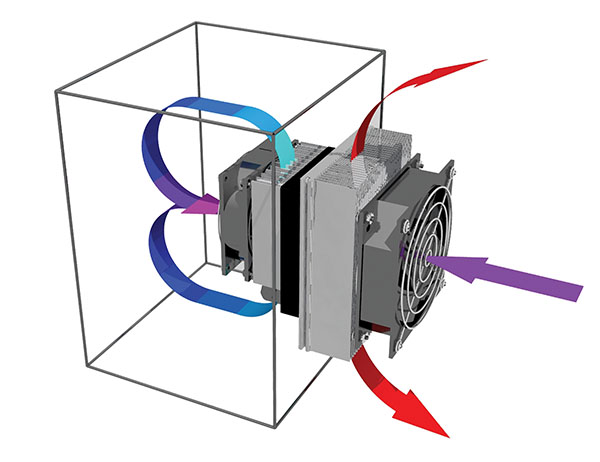
\includegraphics[width=7cm]{camara.jpg}
  	\caption{Sistema térmico, compuesto por una caja negra aislada térmicamente y dos celdas Peltier con sus respectivos disipadores de calor y ventiladores. Recuperado de https://www.thermoelectric.com/air-conditioners/0-100-watts/ahp-250-series/}
	\label{cam_ter}
\end{figure}

\begin{figure}[ht]
  \centering
  	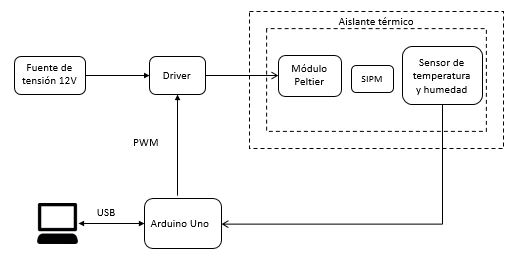
\includegraphics[width=12cm]{Diagrama_Camara.JPG}
  	\caption{Diagrama de bloques del sistema térmico controlado. Este sistema esta compuesto por un un puente H (\textit{ driver}), una caja negra aislada térmicamente donde se encuentra el módulo Peltier, el SIPM y un sensor de temperatura y humedad que se conecta al microcontrolador (Arduino), el microcontrolador envía una señal PWM al puente H en función de la acción de control.}
	\label{Diag_cam}
\end{figure}

\end{itemize} 
\begin{itemize}
\item El segundo módulo es el encargado del acondicionamiento, muestreo, discriminación y digitalización de las señales provenientes del SIPM. En este caso el SIPM se estimula directamente por los fotones generados por la barra centelladora.\\
Como se muestra en la figura \ref{Barra}. Se utiliza una estructura compuesta por una barra centelladora principal y dos barras centelladoras que funcionan como señal de disparo (\textit{trigger}) \cite{Muon_detector_Amiga}. En cada barra centelladora se ubica un SIPM, estos se alimentan con una fuente de tensión controlada suministrada por el fabricante de los SIPM (HAMAMATSU). Los SIPM se ubican sobre una PCB donde se realiza la primera etapa de amplificación.\\
\begin{figure}[ht]
  \centering
  	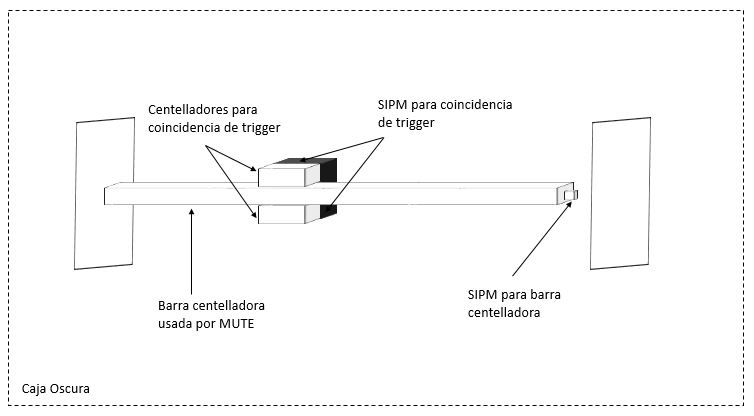
\includegraphics[width=12cm]{Barra.JPG}
  	\caption{Configuración utilizada para medir el numero de p.e. producidos por muón cuando este pasa por una barra centelladora de 120 cm Dos barras centelladoras de 4cm x 4cm x 1cm y dos SIPM se utilizan para generar una señal de disparo por coincidencia.}
	\label{Barra}
\end{figure}
Las señales provenientes de los SIPM, que se encuentran en las barras que generan la señal de disparo, se amplifican e invierten nuevamente, para poder pasar a una etapa de discriminación que consiste en una compuerta AND, la cual cuando las dos señales de disparo se encuentren activas  genera una señal digital que le indica al sistema DAQ que debe realizar la lectura de las señales provenientes del SIPM de la barra principal, como se muestra en la figura \ref{Trigger}. 
\begin{figure}[ht]
  \centering
  	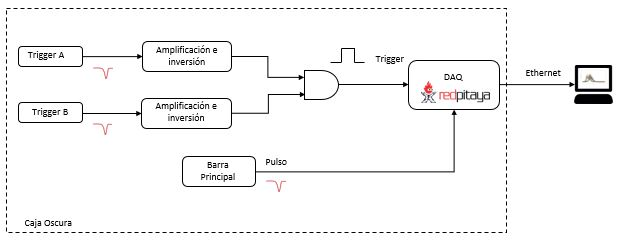
\includegraphics[width=12cm]{Trigger.JPG}
  	\caption{Diagrama de bloques para el sistema de adquisición cuando el SIPM se estimula con los fotones generados por la barra centelladora.}
	\label{Trigger}
\end{figure}

\end{itemize}

\begin{itemize}
\item El tercer módulo se utiliza para la estimulación del SIPM mediante un LED que emite luz de una longitud de onda de $\sim 420nm$, a esta longitud de onda el SIPM tiene su máxima eficiencia \cite{Sipm_S13360_1350CS_datasheet}. Esta señal es controlada en amplitud y duración por un circuito analógico, compuesto por un amplificador comparador y dos potenciómetros. La señal que estimula el LED y la señal de disparo son generadas por una FPGA como se muestra en la figura \ref{LED}. La señal lumínica generada por el LED es conducida mediante una fibra óptica hacia el SIPM, el cual genera pulsos eléctricos que son adquiridos por una plataforma DAQ y enviados a un computador para su posterior procesamiento y análisis \textit{offline}.  


\begin{figure}[ht]
  \centering
  	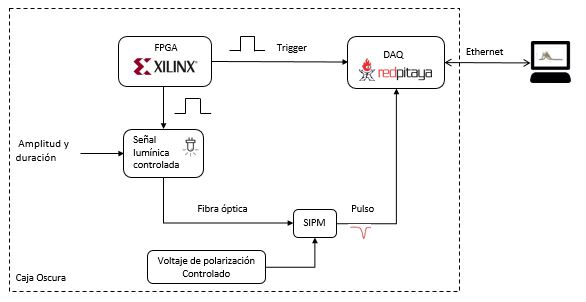
\includegraphics[width=12cm]{Diagrama_led.JPG}
  	\caption{Diagrama de bloques del sistema para la estimulación del SIPM mediante un pulso de luz proveniente de un LED de 420 nm.}
	\label{LED}
\end{figure}

\end{itemize}
  

%%%%%%%%%%%%%%%%%%%%% OBJETIVOS  %%%%%%%%%%%%%%%%%%%%%%%%%%
\newpage

\chapter{Objetivos}
\section{\textbf{Objetivo General}}
 
Diseñar e implementar un sistema de caracterización para los fotomultiplicadores de silicio del telescopio de muones. 

\section{\textbf{Objetivos Específicos}}

\begin{itemize}
    \item Desarrollar los módulos  para las diferentes etapas de caracterización de los SIPM.
    \item  Caracterizar el voltaje de ruptura de los SIPM en función de la temperatura.
	\item Caracterizar el conteo oscuro del SIPM en función de la temperatura.
    \item Evaluar la influencia y la probabilidad del \textit{crosstalk} y \textit{afterpulse} en los eventos registrados desde el SIPM a diferentes temperaturas. 
\end{itemize}


%%%%%%%%%%%%%%%%%%%%% ALCANCES  %%%%%%%%%%%%%%%%%%%%%%%%%%
\newpage
\chapter{Alcances}
En este proyecto de grado se pretende realizar el diseño e implementación de un sistema que permita realizar la caracterización del conjunto de SIPM que componen el hodoscopio de MUTE. \\

La realización de este trabajo tomará como punto de partida la revisión de la literatura técnica disponible, donde se exponen los métodos de caracterización y se muestran los parámetros de rendimiento de los SIPM en detalle. Uno de estos referentes es el detector AMIGA del observatorio Pierre Auger \cite{Muon_detector_Amiga}. \\

El desarrollo del banco de caracterización consiste en la elaboración de los tres módulos que se encuentran en la descripción del trabajo, haciendo claridad que el enfoque principal es el desarrollo de la electrónica necesaria para cada uno de estos módulos, así como en el análisis y procesamiento de los datos adquiridos en el proceso de caracterización. La caracterización de los SIPM comienza con la obtención de la gráfica del voltaje de ruptura en función de la temperatura, que se obtendrá midiendo la corriente oscura del SIPM en función del voltaje de polarización y observando el punto en que ocurre la ruptura para un rango de temperaturas de 0 a 50 $^{\circ}$C, en este proceso se utiliza el sistema térmico controlado. Posteriormente se caracterizan los tipos de ruido que afectan el SIPM, comenzando con el conteo oscuro en función de la temperatura y del voltaje de polarización, luego se mide la frecuencia de ocurrencia del \textit{crosstalk} y por último se calcula la probabilidad de \textit{afterpulse}, para esto se utilizan los módulos dos y tres mencionados en la descripción del trabajo.\\

Todos los resultados obtenidos del proceso de caracterización serán verificados con la literatura y utilizados para realizar el ajuste del voltaje óptimo de operación del sensor. 




%%%%%%%%%%%%%%%%%%%%% JUSTIFICACIÓN  %%%%%%%%%%%%%%%%%%%%%%%%%%
\newpage 
\chapter{Justificación}
Este proyecto surge como parte del proceso de calibración de un telescopio que permitirá la detección del flujo de muones atmosféricos que atraviesan la parte central del volcán Cerro Machín (Tolima), con el fin de estudiar su estructura interna.\\ 
El telescopio está compuesto por dos detectores, un detector Cherenkov en agua y un detector de centelleo (hodoscopio). El hodoscopio esta formado por dos paneles, frontal y posterior, donde se ubican los SIPM que detectan los fotones producidos cuando una partícula cargada atraviesa el material centellador, las partículas que se detectan en este caso son los muones. La información obtenida del hodoscopio permite determinar la trayectoria, el tiempo de vuelo y el flujo de los muones que atraviesan el volcán.\\

Los fabricantes presentan en las hojas de datos algunas de las características ópticas y eléctricas de los SIPM a $25 ^ \circ C$. Sin embargo, al instalar el telescopio en la zona de interés estas características cambian debido a las condiciones meteorológicas del lugar. Por lo anterior, es necesario realizar la  caracterización y calibración de los SIPM que componen el detector. En este proyecto de grado se diseña e implementa un sistema de calibración y caracterización de los SIPM del telescopio de muones (MUTE). 
 
%%%%%%%%%%%%%%%%%%%%% CRONOGRAMA DE ACTIVIDADES%%%%%%%%%%
\newpage 

\chapter{Cronograma de actividades}
A continuación se presenta un calendario de trabajo donde se describen las actividades correspondientes a esta propuesta de investigación.  

\begin{figure}[ht]
  \centering
  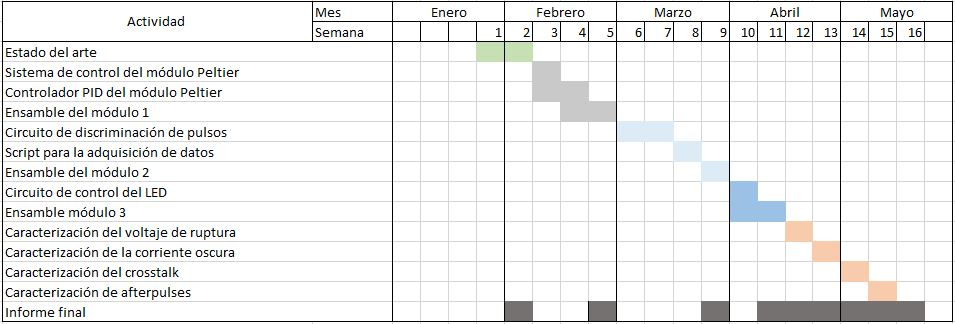
\includegraphics[width=\columnwidth]{Cronograma}
  \caption{Cronograma de actividades.}
\end{figure}

\section{\textbf{Estado del arte}}
En esta etapa se realiza una investigación documental que permita conocer los diferentes trabajos que se han realizado en el área de los detectores de partículas por centelleo más específicamente los que utilizan SIPM, con el fin de realizar una comprensión crítica del fenómeno que permita tener los insumos documentales para la ejecución del plan de trabajo y la elaboración del informe final.  

	\section{\textbf{Sistema de control del módulo Peltier}}
Este circuito está compuesto por un puente H y un microcontrolador Arduino que permiten regular la magnitud y la dirección de la corriente que alimenta las celdas Peltier en respuesta a la acción de control con el fin de aumentar o disminuir la temperatura de la caja oscura dependiendo del punto de ajuste \textit{(set point)}.

	\section{\textbf{Controlador PID del módulo Peltier}}
En esta etapa se diseña el controlador PID, se sintoniza utilizando alguno de los métodos tradicionales y se implementa en el microcontrolador Arduino Uno.

	 \section{\textbf{Ensamble del módulo uno}}
Se ubican los componentes electrónicos y las celdas Peltier en la caja de temperatura, que será una estructura de madera, se realizan las conexiones eléctricas necesarias y se deja el montaje funcional, para el proceso de caracterización.
\section{\textbf{Circuito de discriminación de pulsos}}
Este es un circuito analógico que permite filtrar los pulsos generados por el SIPM, a la vez que los amplifica de tal forma que puedan ser interpretados correctamente por la plataforma de adquisición, este circuito también genera una señal de \textit{trigger} que le indica a la plataforma DAQ cuando se debe realizar la adquisición de datos \cite{Electronica_Amiga}.

    \section{\textbf{\textit{Script} para la adquisición de datos}}
Este \textit{Script} será escrito en el lenguaje \textit{Python} y permitirá la adquisición y el almacenamiento de los pulsos para su posterior procesamiento y análisis \textit{offline}.

	\section{\textbf{Ensamble del módulo dos}}
En esta etapa se ensambla el circuito de discriminación de pulsos y la plataforma de adquisición de datos y se deja el sistema funcional.  

	\section{\textbf{Circuito de control del LED}}
Este es un circuito analógico compuesto por un amplificador operacional en modo comparador y unos potenciometros lineales que permiten generar una señal lumínica controlada en amplitud y duración.   
 
	\section{\textbf{Ensamble del módulo tres}}
Se conecta el circuito de control del LED con la FPA y el sistema DAQ, también se ubica la fibra óptica con el SIPM y se asegura la oscuridad total mediante una caja oscura.  

	 \section{\textbf{Proceso de caracterización del SIPM}}
Este proceso comienza con la caracterización del voltaje de ruptura, que se obtiene a partir de las curvas de corriente en función del voltaje de alimentación del SIPM; así, se realiza un algoritmo para obtener el punto donde la corriente aumente lo suficiente como para asegurar que el SIPM entró en operación \cite{Muon_counting_Amiga}. Finalmente, se puede obtener el voltaje de ruptura para cada una de las temperaturas a las cuales se realizó el procedimiento. En este proceso se utiliza el módulo uno.\\ \\     
Para la caracterización de la corriente oscura se tiene que someter el SIPM a un ambiente de oscuridad total mientas se varia el voltaje de alimentación y se mantiene la temperatura constante, también se pretende obtener el conteo oscuro en función de la temperatura  manteniendo fijo el voltaje de alimentación del SIPM. En este proceso se utiliza el módulo uno.\\ \\ 
La tasa de \textit{crosstalk} se mide contando el número de eventos que se encuentren sobre 1 p.e. por unidad de tiempo, dividiendo esta tasa por la tasa de eventos de 1 p.e se obtiene la probabilidad de \textit{crosstalk}. luego se varia la ganancia del SIPM para obtener la probabilidad de \textit{crosstalk} en función de la ganancia \cite{Measuring_ectr_opti_SIPM_hamamatsu}. En este proceso se utilizan los módulos dos y tres.\\

El cálculo de la probabilidad de \textit{afterpulse} se realiza utilizando el módulo tres, con este se estimula el LED de forma controlada, los \textit{afterpulse} corresponden a los eventos del SIPM que se encuentran fuera del intervalo de tiempo en el que se estimula el LED, como se muestra en la figura \ref{afterpulse}.\\  
\begin{figure}[ht]
  \centering
  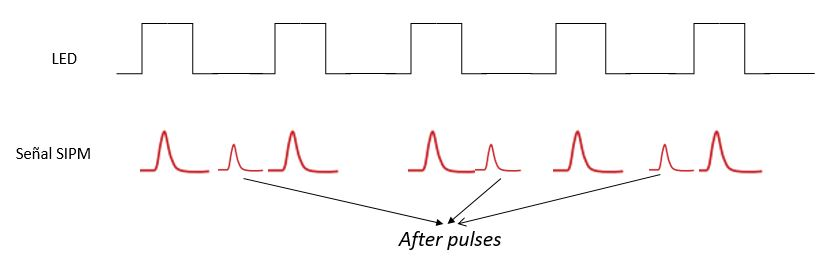
\includegraphics[width=\columnwidth]{Afterpulses}
  \caption{Principio utilizado para la medición de los \textit{afterpulses}. Pulsos emitidos por el LED (linea negra), y la señal generada por el SIPM (linea roja). Los \textit{afterpulses} se generan por electrones que quedan atrapados temporalmente en el material (Silicio) después de una estimulación.}
\label{afterpulse}
\end{figure}

	 \section{\textbf{Informe final}}
Para la realización del informe final se tendrá como insumo los informes parciales realizados en cada una de las etapas del proyecto, donde se documenta el procedimiento realizado, se especifican los diseños utilizados, se muestran los resultados obtenidos y los inconvenientes presentados.   
%%%%%%%%%%%%%%%%%%%%% RECURSOS E INFRAESTRUCTURA %%%%%%%%%%%%%%%%%%%%%%
\newpage 
\chapter{Recursos e Infraestructura}
\section{\textbf{Recursos Humanos}}

\begin{table}[htbp]
\begin{center}
\begin{tabular}{|p{2cm}|p{7cm}|}\hline
%\hline
Función & Descripción \\
\hline    \hline
Director  & Decide sobre los recursos, determina y asigna las tareas. \\ \hline
Codirector  & Decide sobre los recursos, riesgos del proyecto y asigna tareas.  \\ \hline
Autor  & Estudiante de Ingeniería Electrónica encargado de investigar, documentar y ejecutar el proyecto de grado.  \\ \hline
\end{tabular}
\caption{Recursos Humanos.}
\label{Tabla: Recursos Humanos}
\end{center}
\end{table}
 
\section{\textbf{Materiales}}
La lista de los materiales descritos en la tabla \ref{lista_materiales} ya fueron adquiridos por el grupo de investigación GIRG y se encuentran disponibles en el laboratorio del grupo Halley para el desarrollo del proyecto. \\

\begin{table}[htbp]
\begin{center}
\begin{tabular}{|p{2cm}|p{7cm}|}\hline
\hline
Cantidad & Descripción\\
\hline  \hline
30 & Barra centelladora 120 x 4 \textit{cm} \\ \hline
129 & SIPM HAMAMATSU \textit{S13360-1350CS} \\ \hline
1 & FPGA \\ \hline
1 & Red Pitaya\\ \hline
3 & Sensores de temperatura \textit{LM35} \\ \hline
1 & Controlador Arduino uno \\ \hline
1 & Potenciómetro lineal  \\ \hline
2 & Celda Peltier \\ \hline
2 & Ventiladores 12\textit{V DC}\\ \hline
2 & Disipadores de calor  \\ \hline
2 & Fuente regulada de 12 \textit{V} \\ \hline

\end{tabular}
\caption{Materiales}
\label{lista_materiales}
\end{center}
\end{table}
\newpage
%%%%%%%%%%%%%%%%%%%%%%%%% Reseña bibliográfica%%%%%%%%%%%%%%%5
%\chapter{Reseña Bibliográfica}
%\newpage
%%%%%%%%%%%%%%%%%%%%%%%%% Bibliografia %%%%%%%%%%%%%%%%%%%%%5
\cleardoublepage
\addcontentsline{toc}{chapter}{Bibliografía}
%para que aparezca en la tabla de contenidos
\bibliographystyle{unsrt}
\bibliography{Mendeley.bib}
%Archivo con las referencias bibliográficas, creado en JabRef (o manualmente)



\end{document}
